In the previous chapter we introduced the FastSRM algorithm, a framework to
efficiently compute shared responses from the full brain data of multiple
subjects. In this chapter, we
investigate the practical benefits of FastSRM on synthetic and real fMRI data.
FastSRM reduces the fitting time
and memory requirements are reduced considerably, making it possible to compute
shared responses using a laptop in a reasonable amount of time even on
datasets that do not hold in RAM. The efficiency of FastSRM allows us to apply
SRM on a large number of subjects. As an example, we apply FastSRM on 647
subjects from the CamCAN dataset and study how the mixing matrices of the SRM
model are predictive of age.


\section{Comparing Fitting time and performance of FastSRM and
  SRM on synthetic data}
We generate data $\xb_i$ according to the model of Probabilistic SRM. We sample the value of the subject specific noise level from a normal
distribution: $\sigma_i \sim \Ncal(0, 0.1)$. The mixing matrices $A_i$
are obtained by sampling their coefficient from a standardized normal distribution.
Lastly, the covariance of the shared response $\Sigma_s$ is diagonal and the
diagonal values are obtained by sampling from a Dirichlet distribution with
parameter $(1 \dots 1)$.
The number of voxels is fixed to $v=125~000$. The number of samples is given by
$n=1000$. We use $m=10$ subjects and $p=50$ components.

We benchmark different implementations of deterministic SRM and probabilistic
SRM in terms of fitting time and performance. The basic SRM described in
section~\ref{sec:probabilisticsrm} and~\ref{sec:deterministicsrm} is refered to
as \emph{NONE} because no atlas is used. 
\emph{OPTIMAL} is the FastSRM algorithm with optimal atlas which is provably
equivalent to using no atlas. \emph{ReNA} uses the fast clustering approach
of~\cite{hoyos2018recursive} with a number of regions is equal to the number of
components: $r=n$. \emph{PROJ} is the random projection approach that
approximates the optimal reduced data using only $r=5n$ voxels. Lastly
\emph{PCA} applies SRM algorithms to data reduced with a PCA using $r=p+1$
components \textbf{XXX Why  + 1 ? Because of the noise variance I believe we can see ProbSRM as a
  rank $k+1$ model of the data. In practice when the model holds and only $k$
  components are used in the PCA, the noise variance goes to zero and we get numerical errors.}.

For any number of iterations between 1 and 100.
We measure the performance of an algorithm by computing the error between the true component $S \in \RR^{p, n}$ and
the predicted component $\hat{S} \in \RR^{p, n}$ using the quantity:
$\mathrm{mse}(\hat{S}, S) = min_{A \in \RR^{p, p}} \|A \hat{S} - S \|^2_F =  \|S
\hat{S}^{\dagger}\hat{S} - S \|^2_F$. This way of measuring errors is
insensitive to the indeterminacies in DetSRM.
We measure the fitting time in seconds.
Lastly, we measure convergence by computing the gradient $\ell_{\infty}$ norm in
case of DetSRM given by $\max(\mathrm{abs}(G))$ where $G$ is the gradient. For ProbSRM
algorithms the convergence is given by the distance between consecutive values of the loss.

Results are plotted in figure~\ref{fig:srm:synthetic_gradient}. 
We empirically see that the optimal approach is equivalent to using no atlas in
terms of performance. Among approximate methods, the projection
method yields the best results but are quite far away from optimal results.
In general probabilistic methods gives a much better fit than their deterministic
counterpart which shows the superiority of likelihood based methods.
In terms of fitting time, we see that atlas based methods spend most of the time
computing the reduced representation but their total fitting time depends only
weakly on the number of iterations performed. When no atlas is used, the number
of iterations has a very strong impact on performance. The approximate methods
\emph{RENA} and \emph{PROJ} are much faster than other methods but
the \emph{PROJ} one yields much better results. The \emph{PCA} method is
almost as slow as the \emph{OPTIMAL} one while giving much worse results.
Comparing the use of an \emph{OPTIMAL} atlas to using \emph{NONE}, we see that
using the optimal atlas is faster as long as the number of iterations is greater
than $30$.
Looking at the convergence curves, we see that even after $100$ iterations, algorithms did
not fully converge. This means that in practice a much larger number of
iterations is needed which justifies why the \emph{OPTIMAL} atlas method is better.
Lastly, when the time budget is very tight, using an approximate atlas with the
\emph{PROJ} method is a better choice than
using SRM with less iterations. 

\begin{figure}
  \centering
  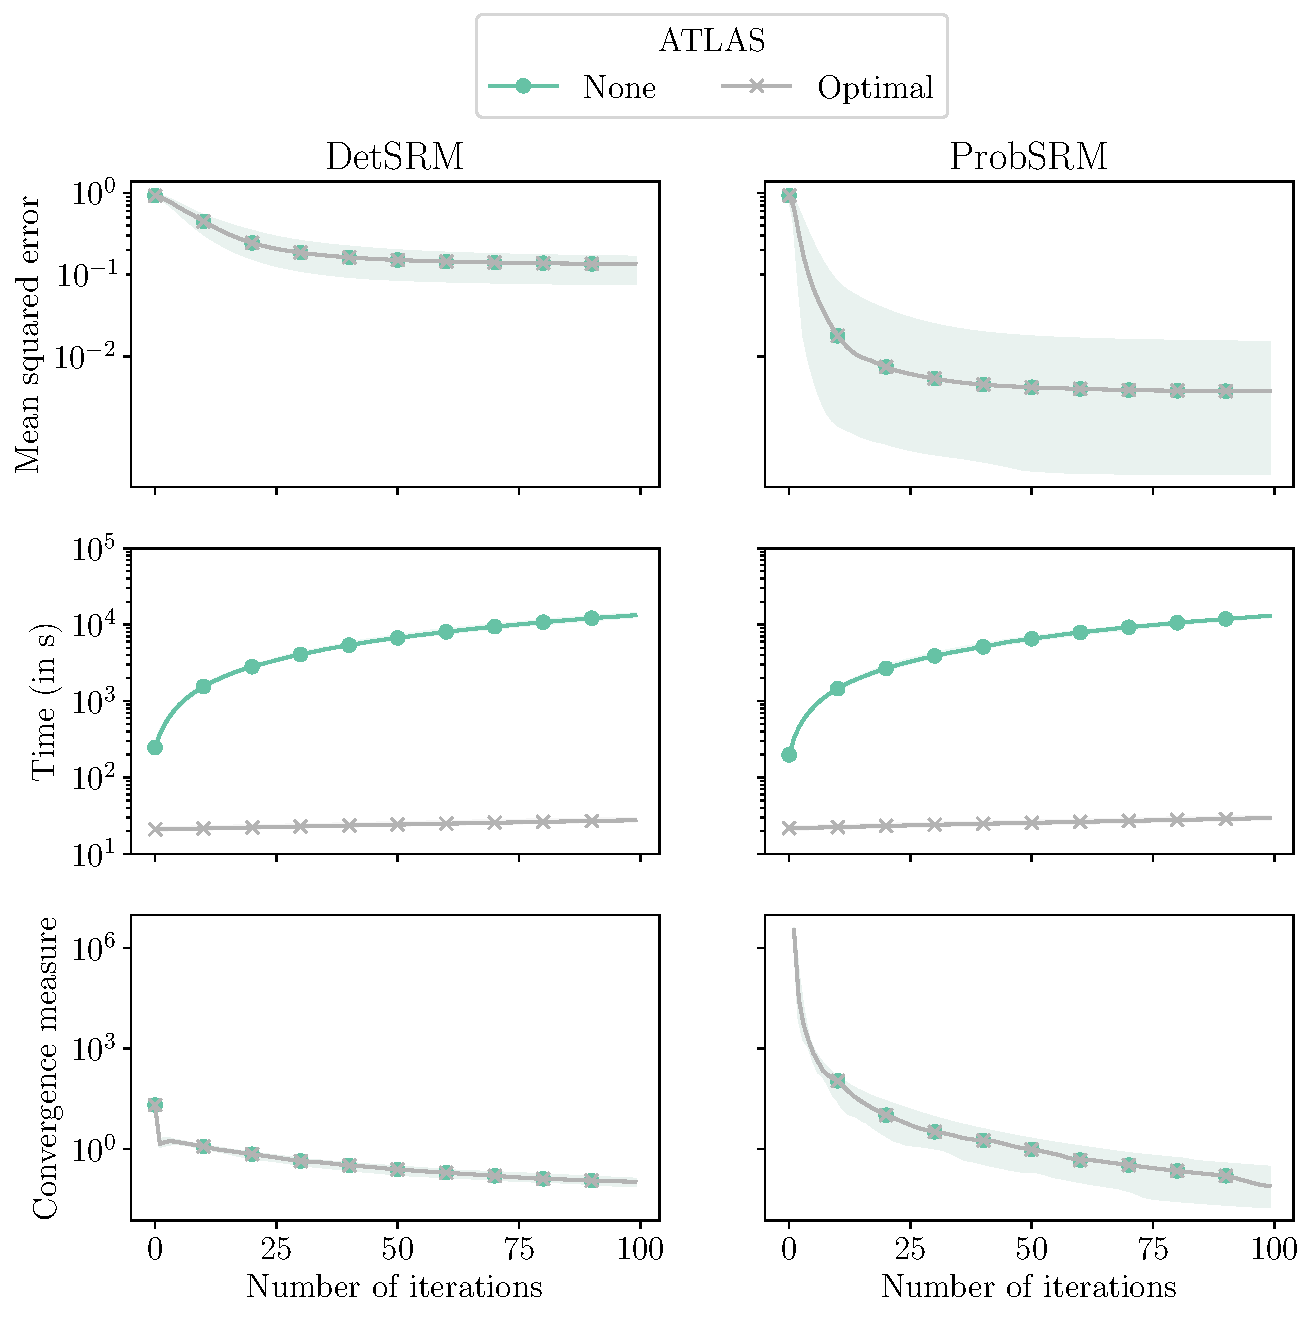
\includegraphics[width=\textwidth]{figures/srm/synthetic_gradient.pdf}
  \caption{\textbf{Benchmark of SRM algorithms on synthetic data: } Performance,
    fitting time and convergence of SRM algorithms (left) Deterministic SRM
    (right) Probabilistic SRM.  As expected, the FastSRM with optimal atlas matches the performance of standard SRM algorithms and is faster when the number of
    iterations is larger than 30. We can see that after 30 iterations,
    convergence is far from being reached. PROJ is the best approximate atlas
    yielding in the probabilistic case a similar solution than what would have
    been obtained using 10 iterations of ProbSRM while being much faster.}
  \label{fig:srm:synthetic_gradient}
\end{figure}

\section{Experiments on fMRI data}
We evaluate the performance of FastSRM on three fMRI datasets of subjects
exposed to naturalistic stimuli: Sherlock, Forrest and CamCAN (more details
about these datasets are available in section~\ref{srm:datasets:fmri}).
\subsection{Comparing fitting time, memory usage and performance on a
  timesegment matching experiment}
\label{sec:timesegment_expe}
\label{timesegment_expe}
The timesegment matching experiment is first introduced
in~\cite{chen2015reduced}.
In a nutshell, the time-segment matching accuracy measures the similarity between two multivariate time-series by trying to localize a time-segment in one time-series by correlation with the other.
In the context of movie watching this measure has a lot of sense: if we split
the movies in various parts and compute two representations of each part, it makes
sense that the representation corresponding to the same parts are closer than
the representation corresponding to different parts. 
This explains why timesegment matching is a standard evaluation of SRM-like methods also used in  \cite{chen2015reduced}, \cite{guntupalli2018computational}, \cite{Nastase741975} or
\cite{zhang2016searchlight}.

We now describe more precisely the experimental design.
We split the runs into a train and test set. After fitting the model on the
training set, we apply the unmixing matrices $W_i=A_i^{-1}$ of each subject on the test set yielding individual components matrices. We estimate the shared responses by averaging the individual components of each subjects but one.  We select a target time-segment (9 consecutive timeframes) in the shared responses and try to localize the corresponding time segment in the components of the left-out subject using a maximum-correlation classifier.
The time-segment is said to be
correctly classified if the correlation between the sample and target
time-segment is higher than with any other time-segment (partially overlapping time windows are excluded).
% 
We use 5-Fold cross-validation across runs: the training set contains 80\% of the runs and the test set 20\%, and repeat the experiment using all possible choices for left-out subjects. 
% 
The mean accuracy is reported in Figure~\ref{fig:timesegment} (bottom). 
% 

We would like to highlight here that these experiments are not exactly the same
as in~\cite{chen2015reduced} as we use full brain data and they use regions of
interest. However, the code used for this experiment is very similar to the tutorial in \url{https://brainiak.org/tutorials/11-SRM/}.

\subsection{Predict age from spatial components}
Since spatial components are subject-specific they should be predictive of subject-specific features such as age.
%
In this experiment we try to predict subject's age from movie-watching data using SRM algorithms.
%
Functionally matched spatial components are obtained using an SRM algorithm.
%
They are divided into two groups (train and test data) where the train set contains 80\% of the data and the test set 20\%.
%
Within the train set we split again our data into two groups: the first group is used to train one Ridge model per spatial components, the second group is used to train a Random Forest to predict age from Ridge predictions. This way of stacking models is similar to the pipeline used in \cite{rahim2017joint}.
%
We use 5 fold cross validation to split the train set (so that the number of samples used to train the Random Forest is the number of elements in the train set).
%
Then the train set is used to train one Ridge model per spatial component.
%
On the test set each Ridge model makes a prediction and the predictions are aggregated using the Random Forest model.
%
An illustration of the process is available in Figure~\ref{fig:experiment_age_prediction}. 

In each Ridge model, the coefficient that determines the level of l2 penalization is set by generalized cross validation, an efficient form of leave-one-out cross validation (see the RidgeCV implementation of Scikit Learn \cite{pedregosa2011scikit}).

The train and test sets are chosen randomly. 5 different choices for the train and test set are made. We report the average mean absolute error (MAE) on the test set averaged over the 5 splits.

\begin{figure}
\centering
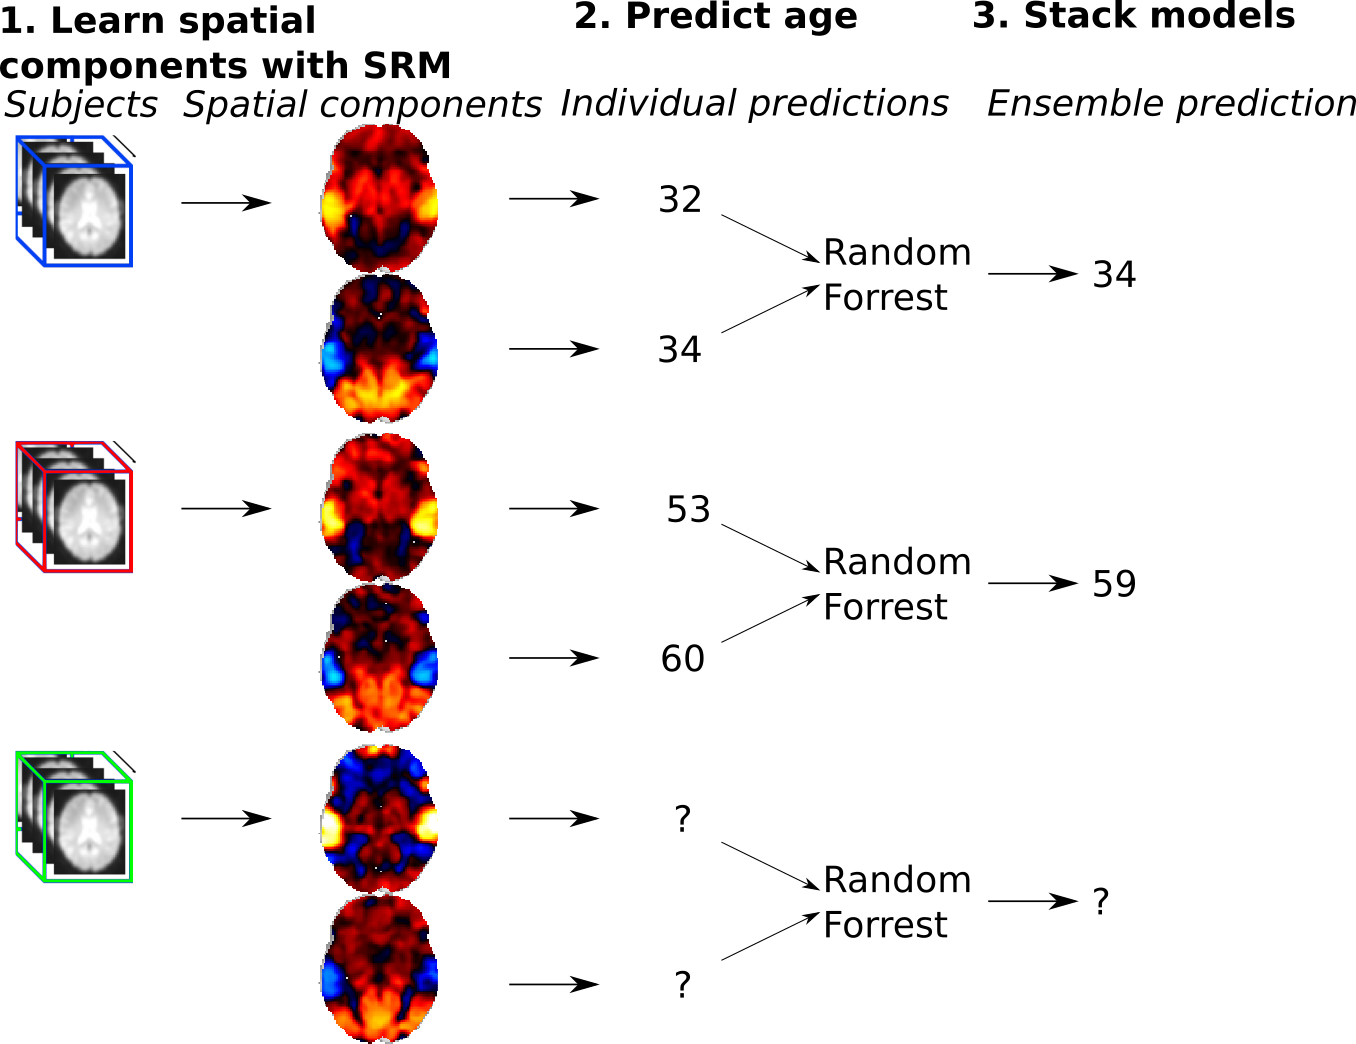
\includegraphics[scale=0.35]{figures/srm/conceptual_figure72.png}
\caption{\textbf{Experiment — Predict age from spatial components extracted using FastSRM}: We first learn the spatial components from fMRI data using SRM. We learn one Ridge model per spatial components to predict age across subjects. Then, these models are aggregated using a Random Forest (like in \cite{rahim2017joint}).} 
\label{fig:experiment_age_prediction}
\end{figure}


Because FastSRM is fast and memory efficient, it enables large-scale analysis of fMRI recordings of subjects exposed to the same naturalistic stimuli.
%
We use all 647 subjects of the CamCAN dataset and demonstrate the usefulness of FastSRM by showing that the spatial components that it extracts from movie watching data are predictive of age.
%
A key asset of FastSRM is that these spatial components can be visualized and therefore provide meaningful insights. 

Figure~\ref{fig:predict_age} shows that FastSRM predicts age with a good accuracy (better than ProbSRM and a lot better than chance) resulting in a mean absolute error (MAE) of 7.5 years.
%
It also shows that on CamCAN data, FastSRM is 4x faster and more than 150x more memory efficient than ProbSRM. As before and in order to ensure fair comparison the number of iterations is set to $10$ and we do not make use of parallelization. Note that the memory requirements of ProbSRM on the CamCAN dataset (186Go) make it difficult to use.
%
FastSRM does not suffer from memory issues, making it suitable to analyse big datasets.

A key asset of our pipeline is that we can see which spatial components are most predictive of age by using feature importance.
%
Feature importance is assessed by the Gini importance defined in \cite{breiman2001random} or \cite{louppe2013understanding}.
%
It measures for each feature the relative reduction in Gini impurity brought by this feature.
%
Feature importance varies with different splits. We use the averaged feature importance over the 5 splits of our pipeline.
%
In Figure~\ref{fig:predict_age} are shown the 3 most important spatial components representing respectively 16\%, 12\% and 8\% of total feature importance.
%
These spatial components in decreasing order of importance represent the visual dorsal pathway, the precuneus and the visual ventral pathway. 
%
The fact that averaged spatial components are interpretable and meaningful allows us to study the influence of age on brain networks involved in movie-watching.
%
In Figure~\ref{fig:predict_age_interpretation}, we plot the most important spatial component averaged within groups of ages.
%
We see that these spatial components evolve with age allowing us to visually identify which regions are meaningful. 
%
It turns out that aging is mostly reflected in brain activity as a
fading of activity in the spatial correlates of movie watching,
particularly in the dorsal visual cortex.


\begin{figure}
\centering
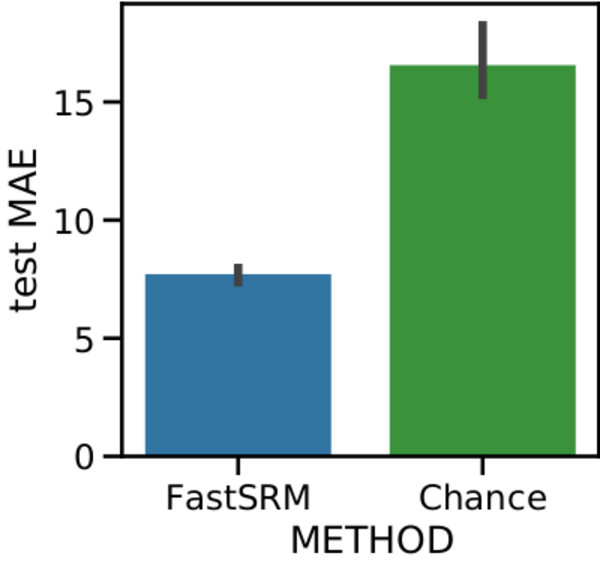
\includegraphics[scale=0.44]{figures/srm/predict_age.pdf}

\begin{tabular}{|c|c|c|}
	\hline
	Algorithm & Memory usage (in Go) & Fitting time (in minutes) \\
	\hline
	FastSRM & 1.1 & 15 \\
	ProbSRM & 186.3 & 69 \\
	\hline
\end{tabular}
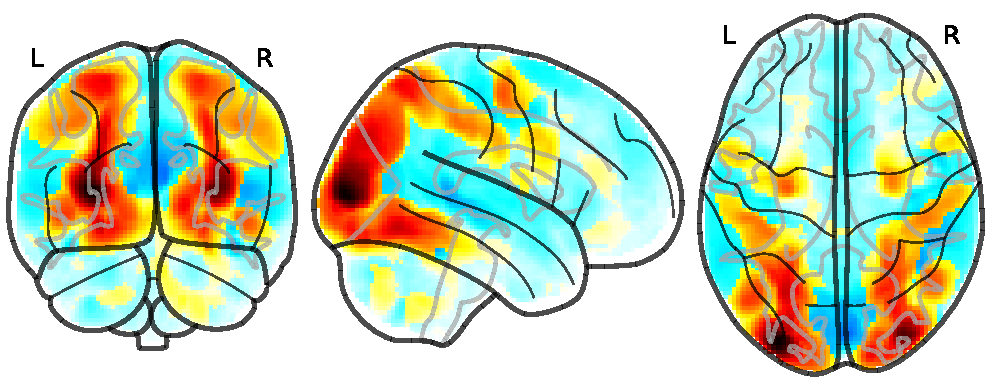
\includegraphics[scale=0.365]{./figures/srm/maps_feature_imp_0_16.pdf}
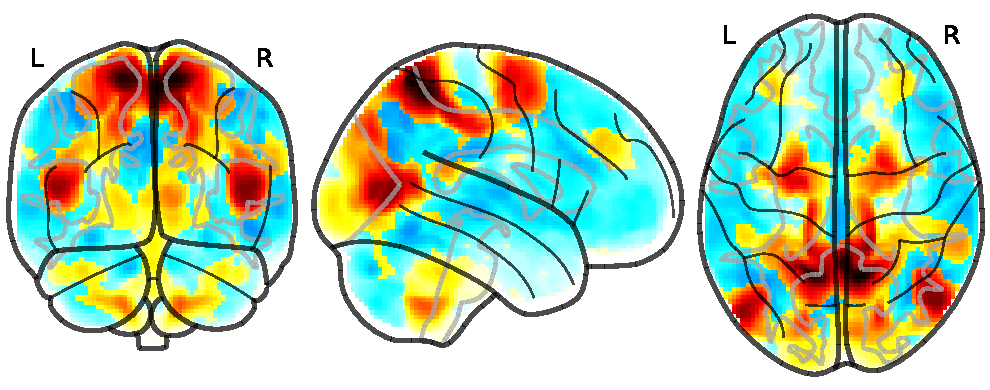
\includegraphics[scale=0.365]{./figures/srm/maps_feature_imp_0_12.pdf}
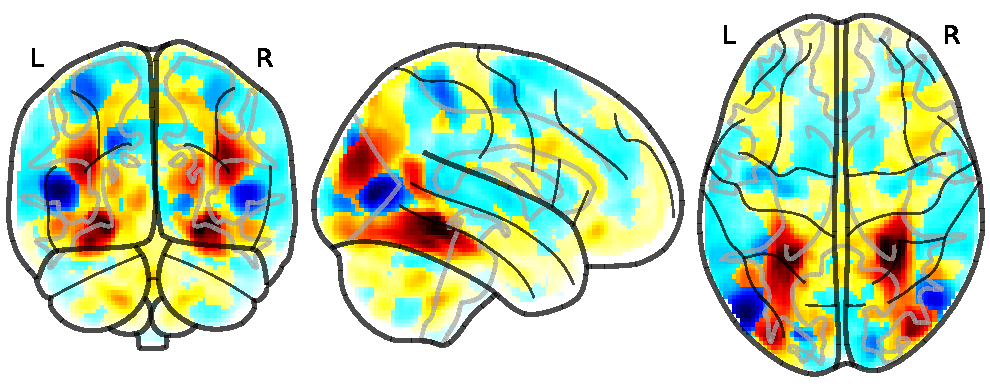
\includegraphics[scale=0.365]{./figures/srm/maps_feature_imp_0_08.pdf}

\caption{\textbf{Age prediction from spatial components}: (top) FastSRM predicts age with a good accuracy (better than ProbSRM and a lot better than chance) resulting in a mean absolute error (MAE) of 7.5 years. (middle) FastSRM is more than 4x faster than ProbSRM and uses 150x less memory, hence it scales better than ProbSRM. (bottom) The three most important spatial components in terms of the reduction in Gini impurity they bring (see Gini importance or Feature importance in \cite{breiman2001random}, \cite{louppe2013understanding}). From top to bottom, the most important spatial component (feature importance: 16\%) highlights the visual dorsal pathway, the second most important spatial component (feature importance: 12\%) highlights the precuneus and the third most important spatial component (feature importance: 8\%) highlights the visual ventral pathway.} 
\label{fig:predict_age}
\end{figure}

\begin{figure}
\centering
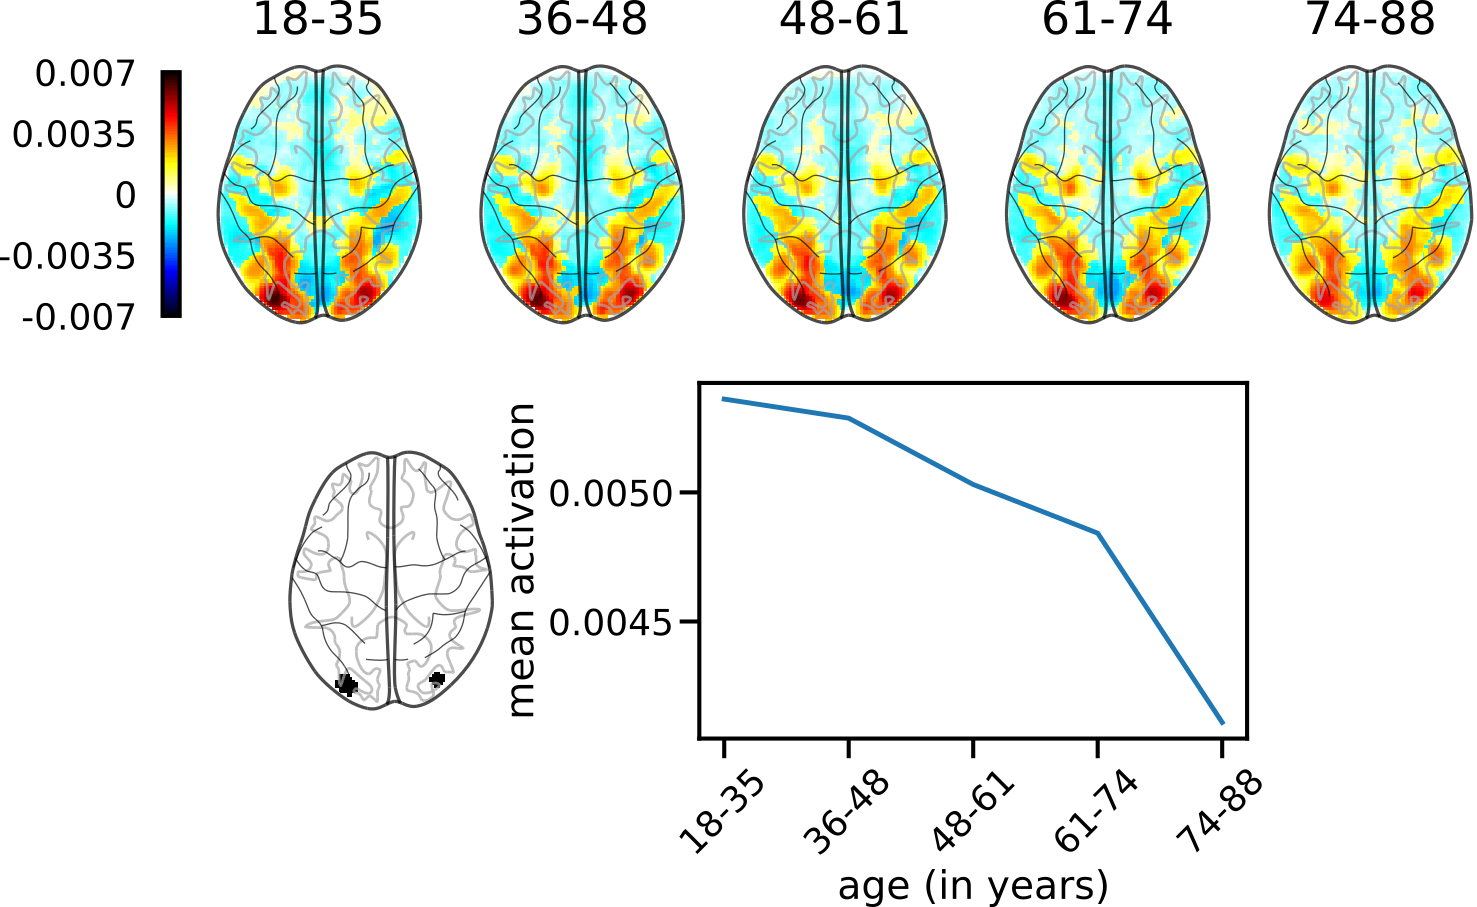
\includegraphics[scale=0.35]{figures/srm/feature_importance_age_prediction.png}
\caption{\textbf{Evolution of the most predictive spatial component with age}: (Top) Spatial component most predictive of age averaged within groups of different age (18-35, 36-48, 48-61, 61-74, 74-88). (Bottom) Mean activation in the region highlighted by the mask on the left. We see that the activity in the dorsal pathway decreases with age, which explains why this spatial component is a good predictor of age.}
\label{fig:predict_age_interpretation}
\end{figure}



\section{Results and Discussion}

\subsection{Conclusion}
As studies using naturalistic stimuli will tend to become more common and large within and across subjects, we need scalable models especially in terms of memory usage.
%
This is what FastSRM provides.
%
We show that while FastSRM matches the performance of standard SRM implementations, it is
significantly faster and requires a lot less memory.

FastSRM allows large scale analysis of fMRI data of subjects exposed to naturalistic stimuli. As one example of such analysis, we show that it can be used to predict age from movie-watching data. Interestingly, although FastSRM is an unsupervised model, it extracts meaningful networks and as such constitutes a practical way of studying subjects exposed to naturalistic stimuli.

We also show that individual information can be extracted from the fMRI activity when subjects are exposed to naturalistic stimuli. Our predictive model is reminiscent of that of \cite{bijsterbosch2018relationship}, that have shown that ICA components obtained from the decomposition of resting state data carry important information on individual characteristics. 
%

As a side note, we chose to keep the orthonormality assumptions of the original SRM model but slight modifications of our implementation of FastSRM would allow one to build more refined model promoting sparsity, non-negativity or smoothness of spatial components for example.

The remaining difficulty with SRM is to interpret the spatio-temporal decomposition. Reverse correlation \cite{hasson2004intersubject} can be used to clarify the cognitive information captured in the shared response.